% ---------------------------------------------------------------
% Section: Physics Model Selection
% ---------------------------------------------------------------

\section[Physics Model Selection]{Physics Model Selection: Is Plain ABP Enough?}

\begin{frame}{ABP Is a Null Model}
\begin{columns}
\begin{column}{0.58\textwidth}
\begin{figure}
    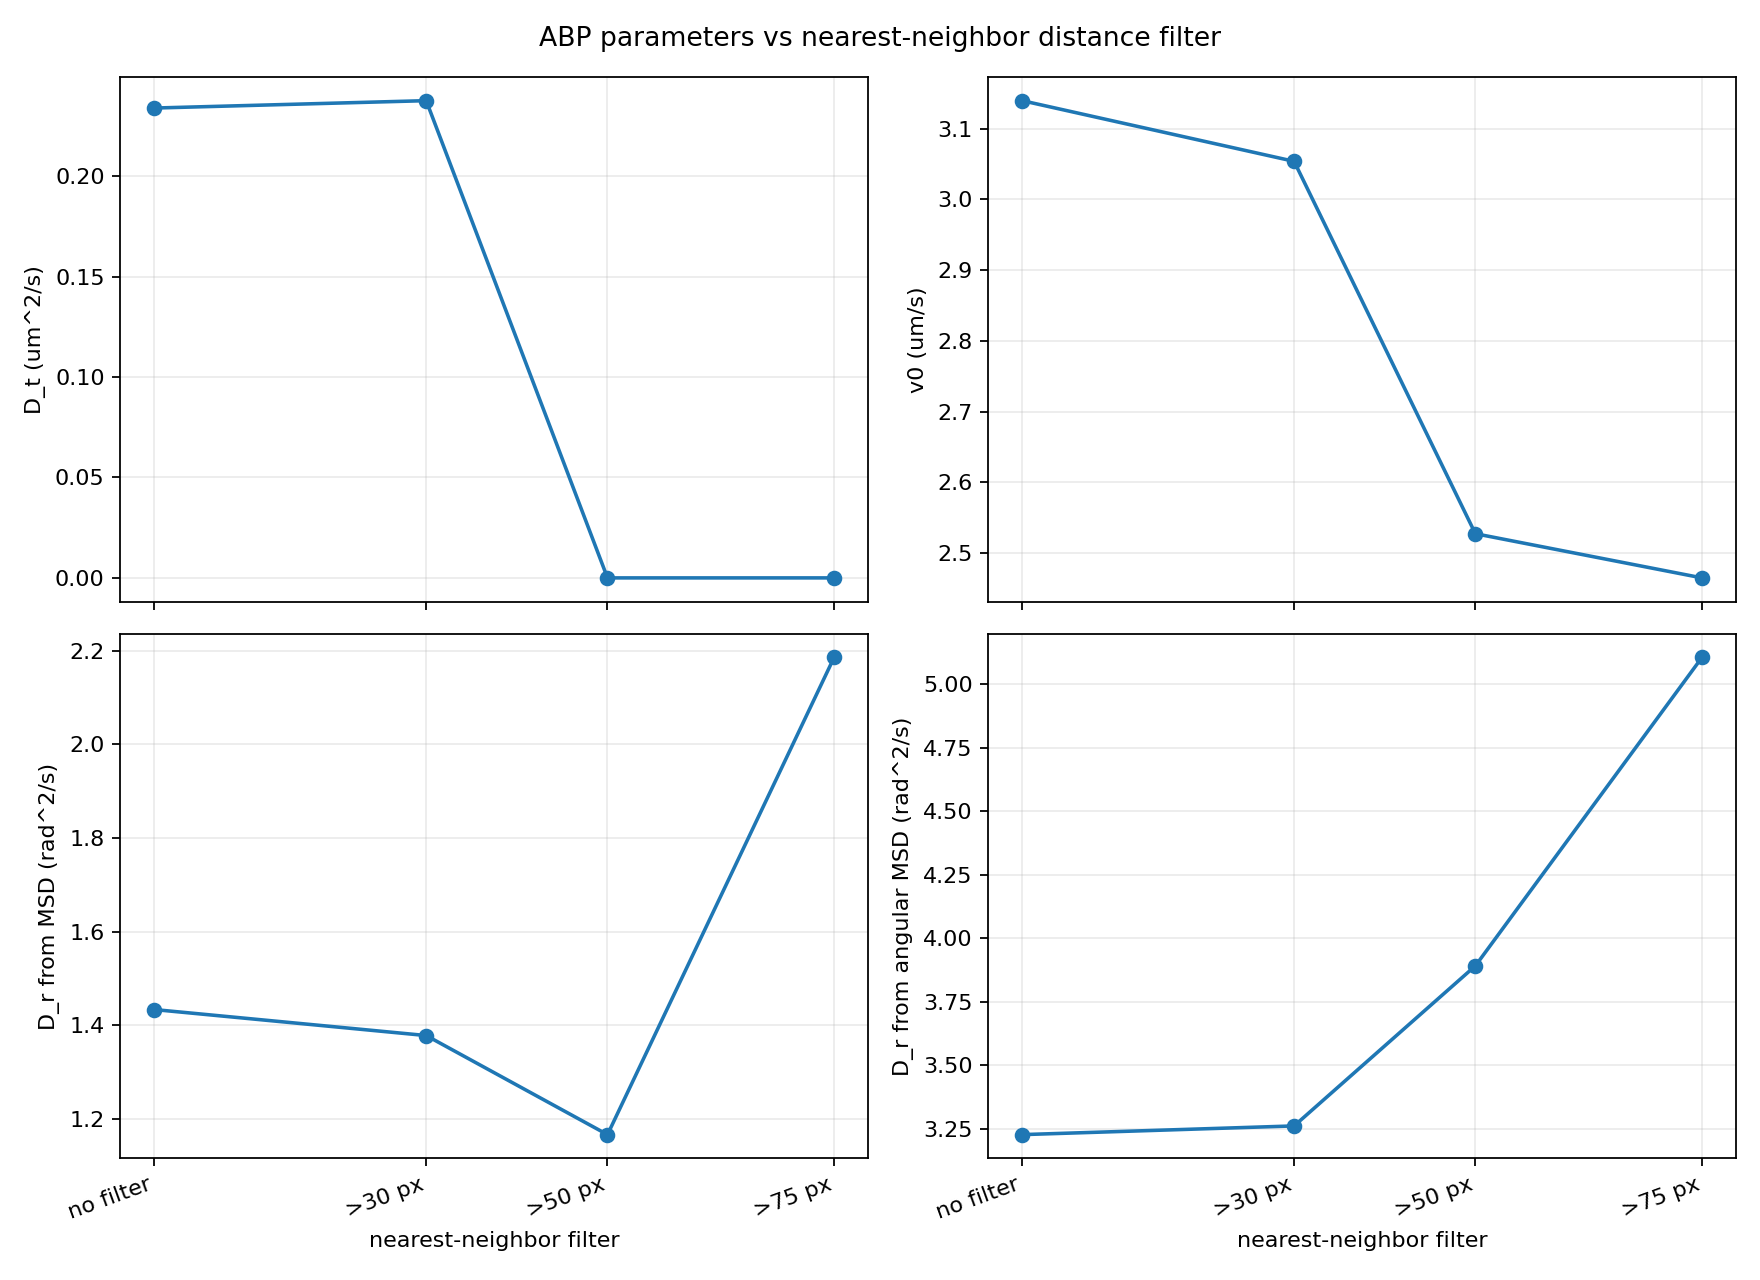
\includegraphics[width=\textwidth]{imglib/progress_update/filtered_abp_parameters.png}
\end{figure}
\end{column}
\begin{column}{0.42\textwidth}
\begin{myalert}[Main result]
\small ABP parameters drift strongly after neighbour filtering; one global ABP fit is not a stable description of the full dataset.
\end{myalert}
\smallskip
\begin{mynote}
\footnotesize At nn$>$50 px only 58\% of states remain; at nn$>$75 px only 21\%.
\end{mynote}
\end{column}
\end{columns}
\end{frame}

\begin{frame}{Interaction Filtering Changes the Curves}
\begin{figure}
    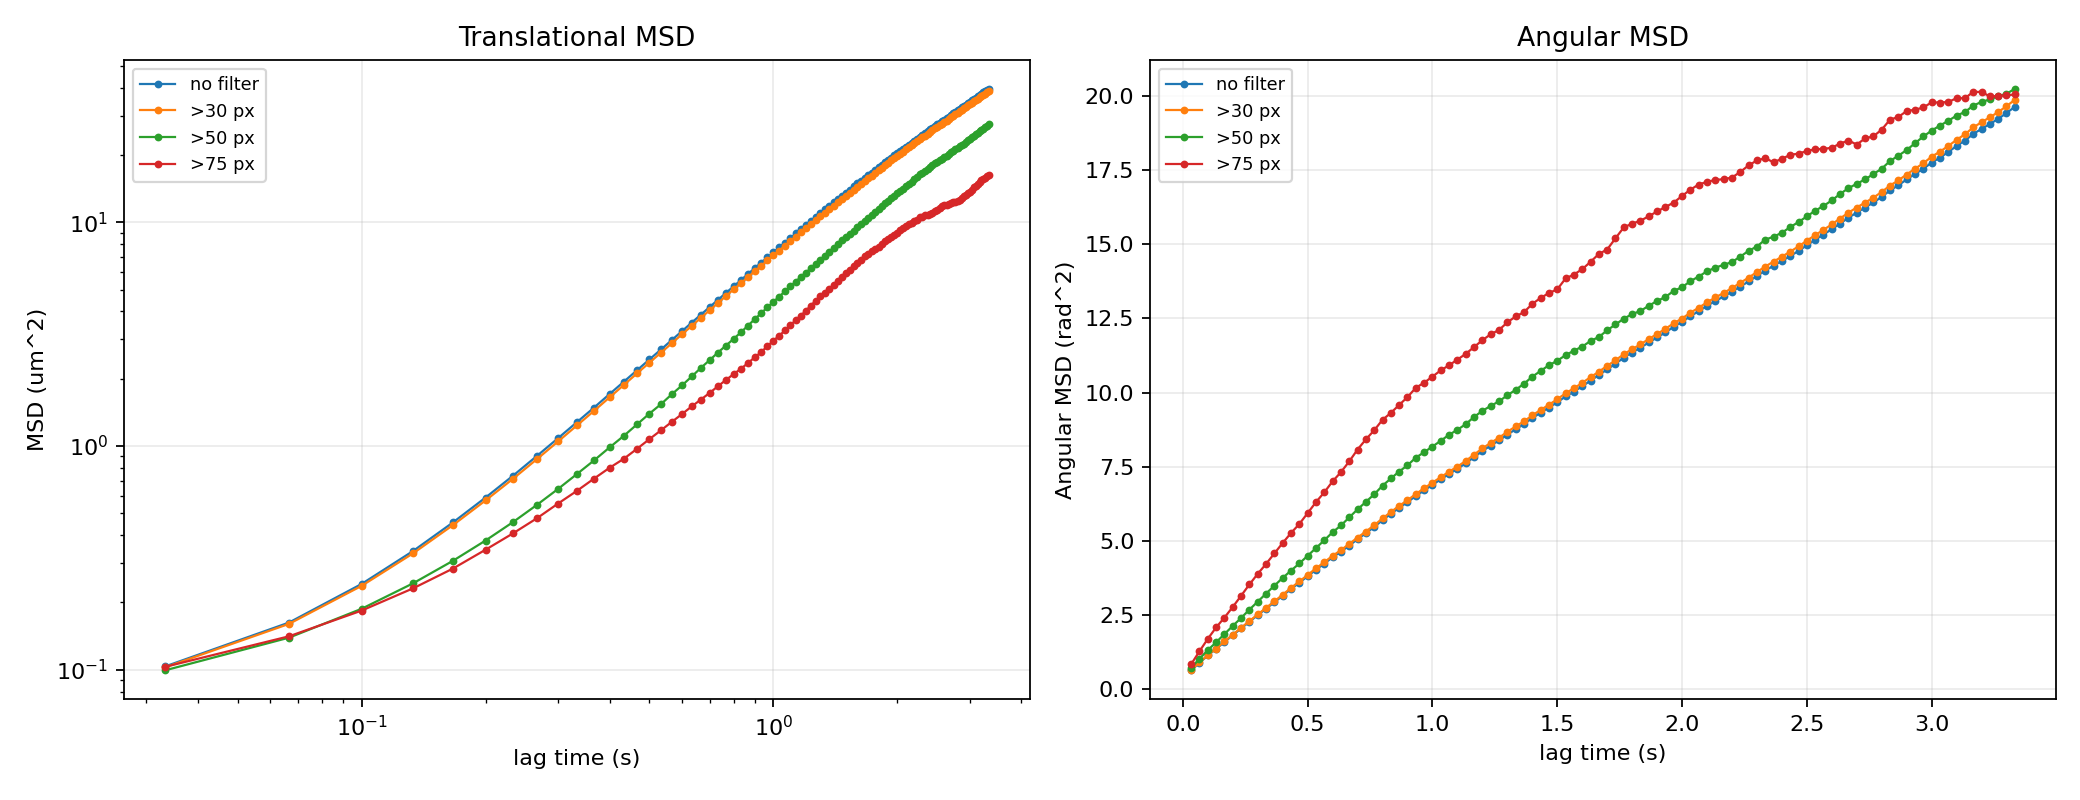
\includegraphics[width=\textwidth, height=0.78\textheight, keepaspectratio]{imglib/progress_update/filtered_abp_msd_curves.png}
\end{figure}
\end{frame}

\begin{frame}{Velocity Persistence Is Short}
\begin{columns}
\begin{column}{0.62\textwidth}
\begin{figure}
    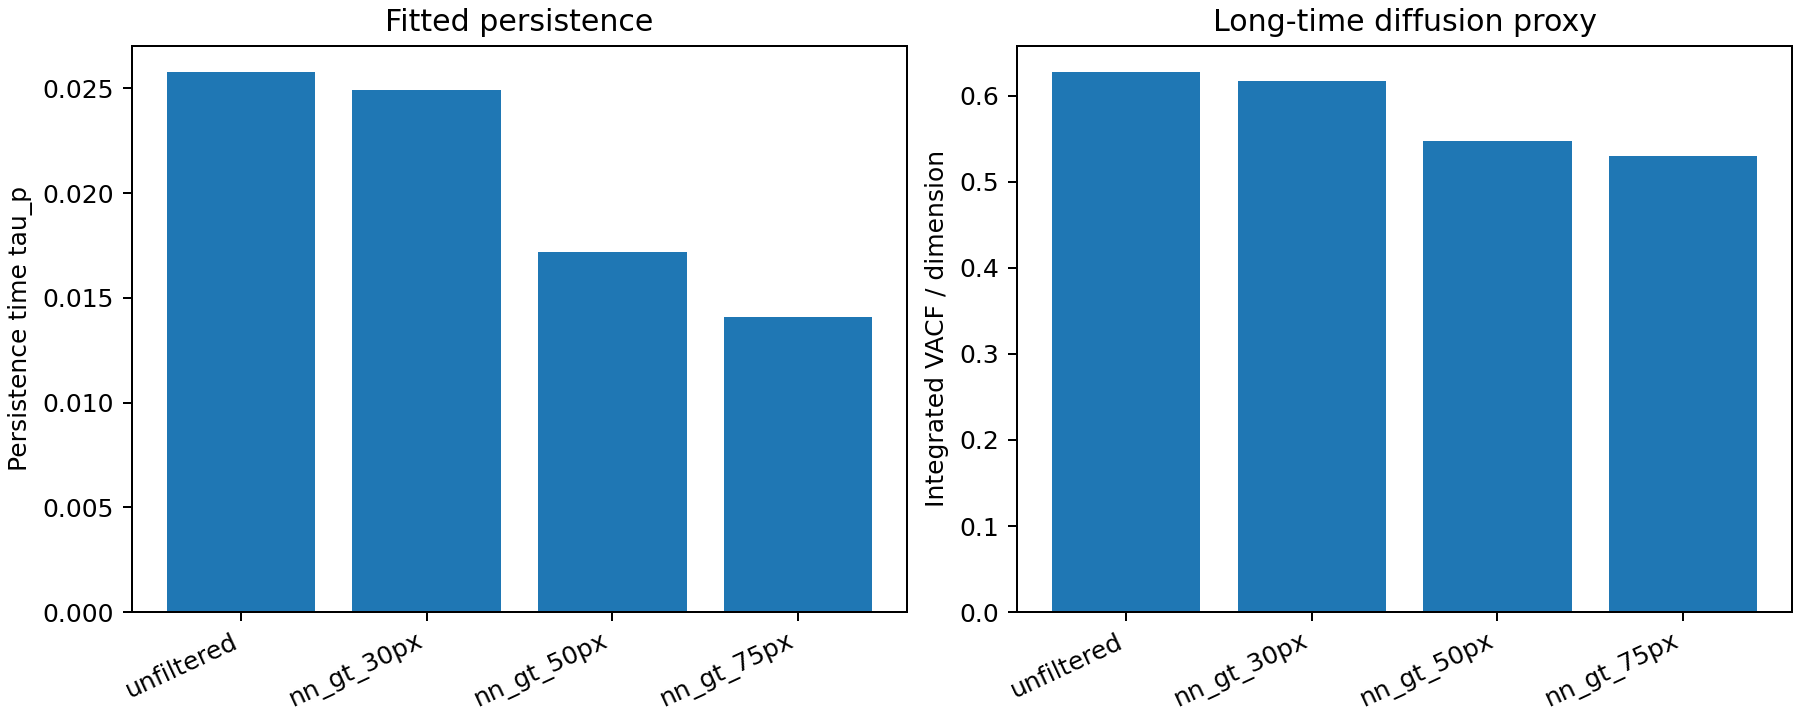
\includegraphics[width=\textwidth]{imglib/progress_update/velocity_persistence_summary.png}
\end{figure}
\end{column}
\begin{column}{0.38\textwidth}
\begin{myalert}[Finding]
\small $\tau_p < 1$ frame at 30 fps, and it shrinks under stricter neighbour filtering.
\end{myalert}
\smallskip
\begin{mynote}
\footnotesize A clean long-persistence ABP picture is questionable for these tracks.
\end{mynote}
\end{column}
\end{columns}
\end{frame}

\begin{frame}{Central Drift / Confinement}
\begin{columns}
\begin{column}{0.5\textwidth}
\begin{figure}
    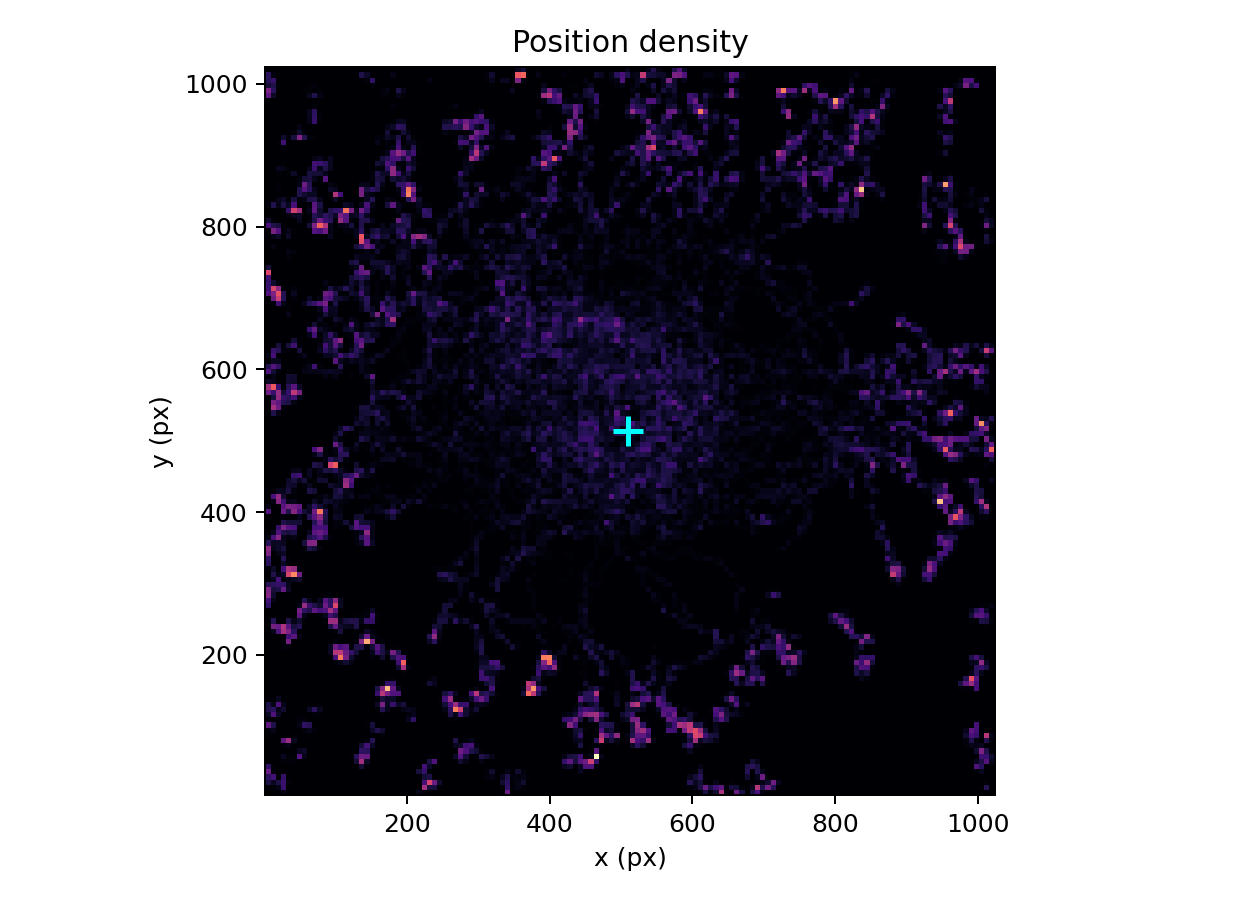
\includegraphics[width=\textwidth, height=0.54\textheight, keepaspectratio]{imglib/progress_update/confinement_position_density.png}
\end{figure}
\end{column}
\begin{column}{0.5\textwidth}
\begin{figure}
    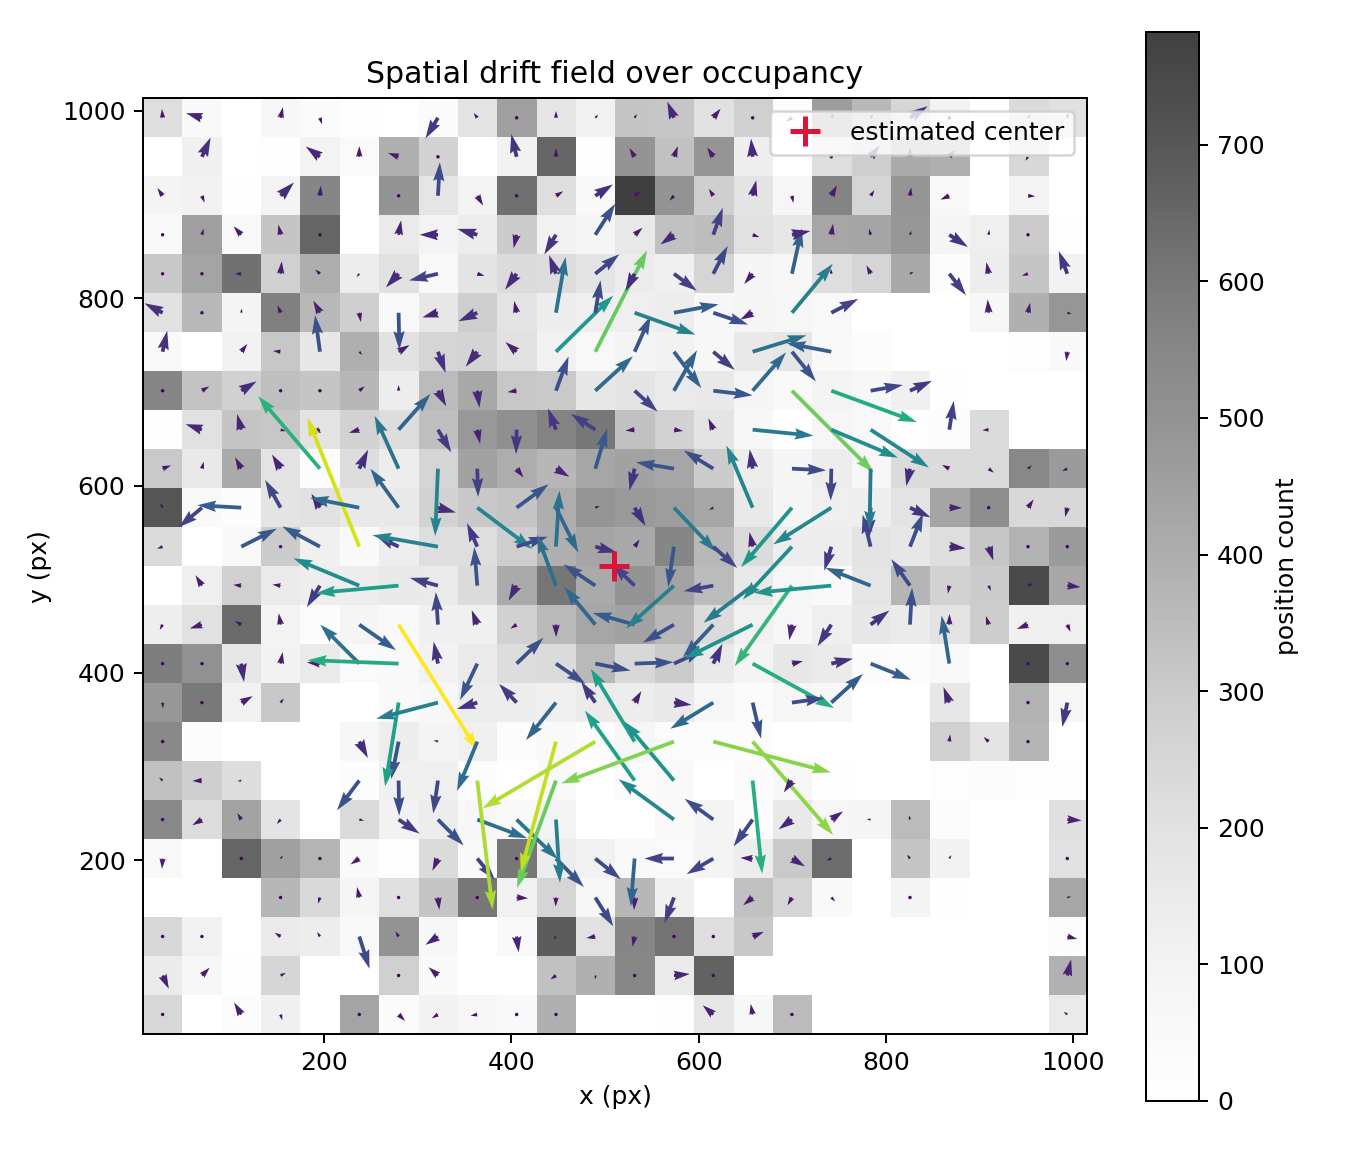
\includegraphics[width=\textwidth, height=0.54\textheight, keepaspectratio]{imglib/progress_update/confinement_quiver_drift_field.png}
\end{figure}
\end{column}
\end{columns}
\vspace{-0.8em}
\begin{mynote}
\scriptsize Drift is measurable, but interaction filtering should precede fitting a global central-potential term.
\end{mynote}
\end{frame}

\begin{frame}{Radial Diagnostics}
\begin{columns}
\begin{column}{0.5\textwidth}
\begin{figure}
    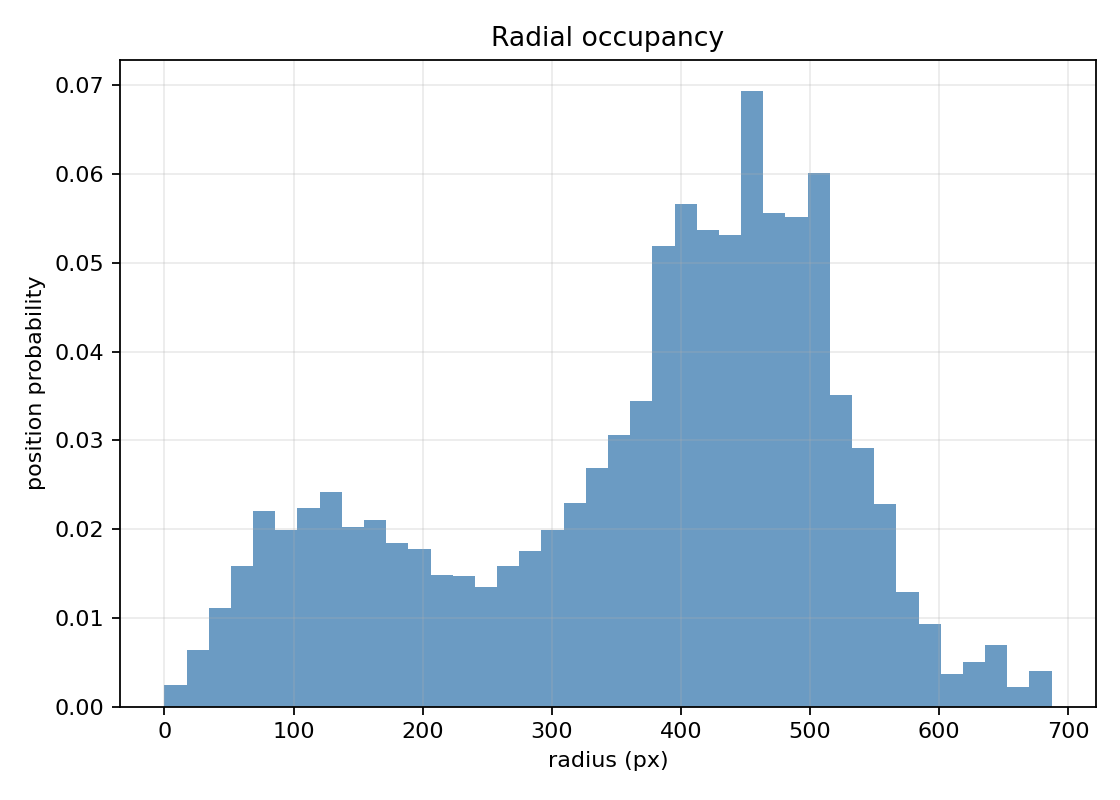
\includegraphics[width=\textwidth]{imglib/progress_update/confinement_radial_occupancy.png}
\end{figure}
\end{column}
\begin{column}{0.5\textwidth}
\begin{figure}
    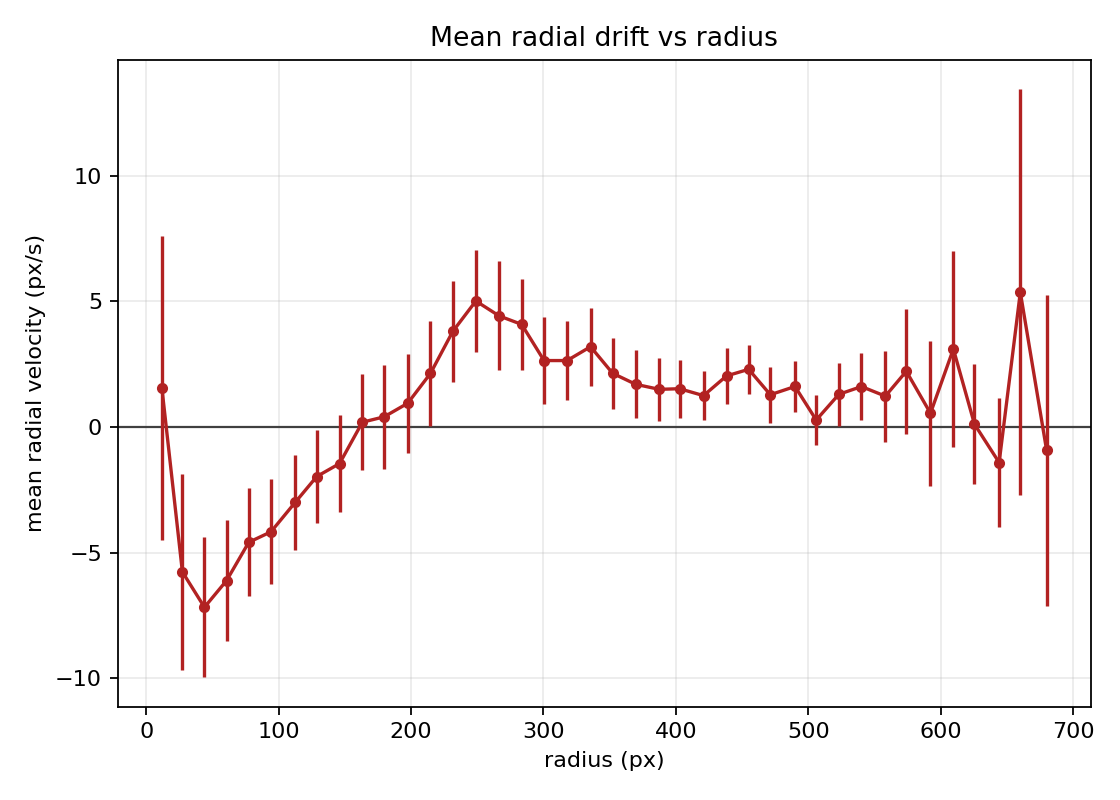
\includegraphics[width=\textwidth]{imglib/progress_update/confinement_mean_radial_velocity_vs_radius.png}
\end{figure}
\end{column}
\end{columns}
\end{frame}

\begin{frame}{Raw Motion Statistics}
\begin{columns}
\begin{column}{0.5\textwidth}
\begin{figure}
    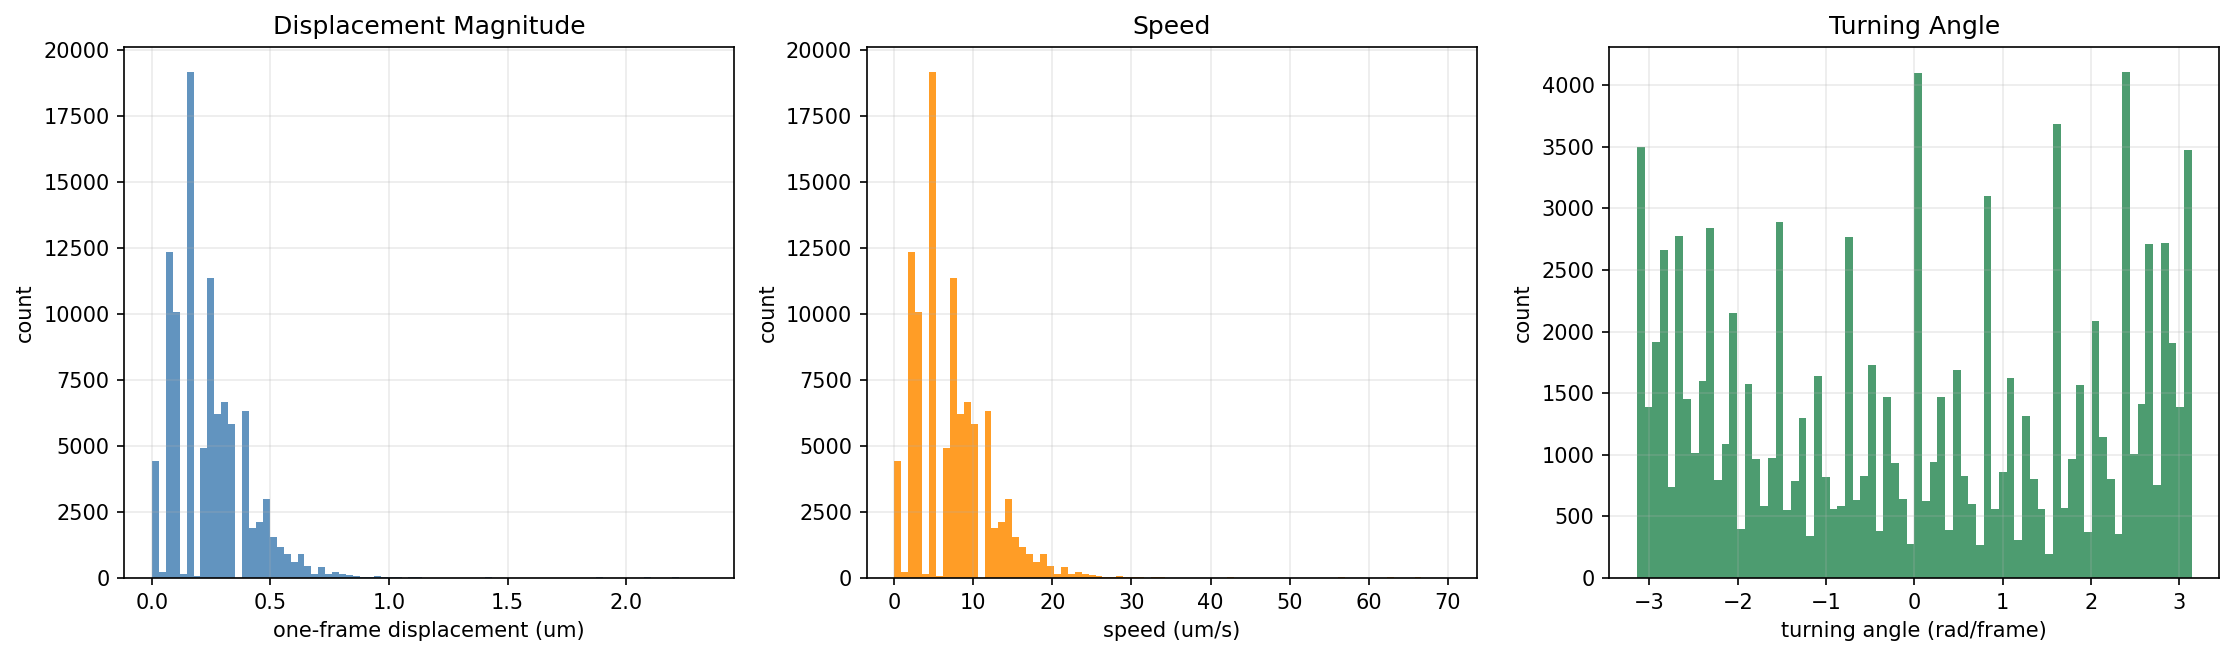
\includegraphics[width=\textwidth]{imglib/progress_update/motion_real_only_distributions.png}
\end{figure}
\end{column}
\begin{column}{0.5\textwidth}
\begin{figure}
    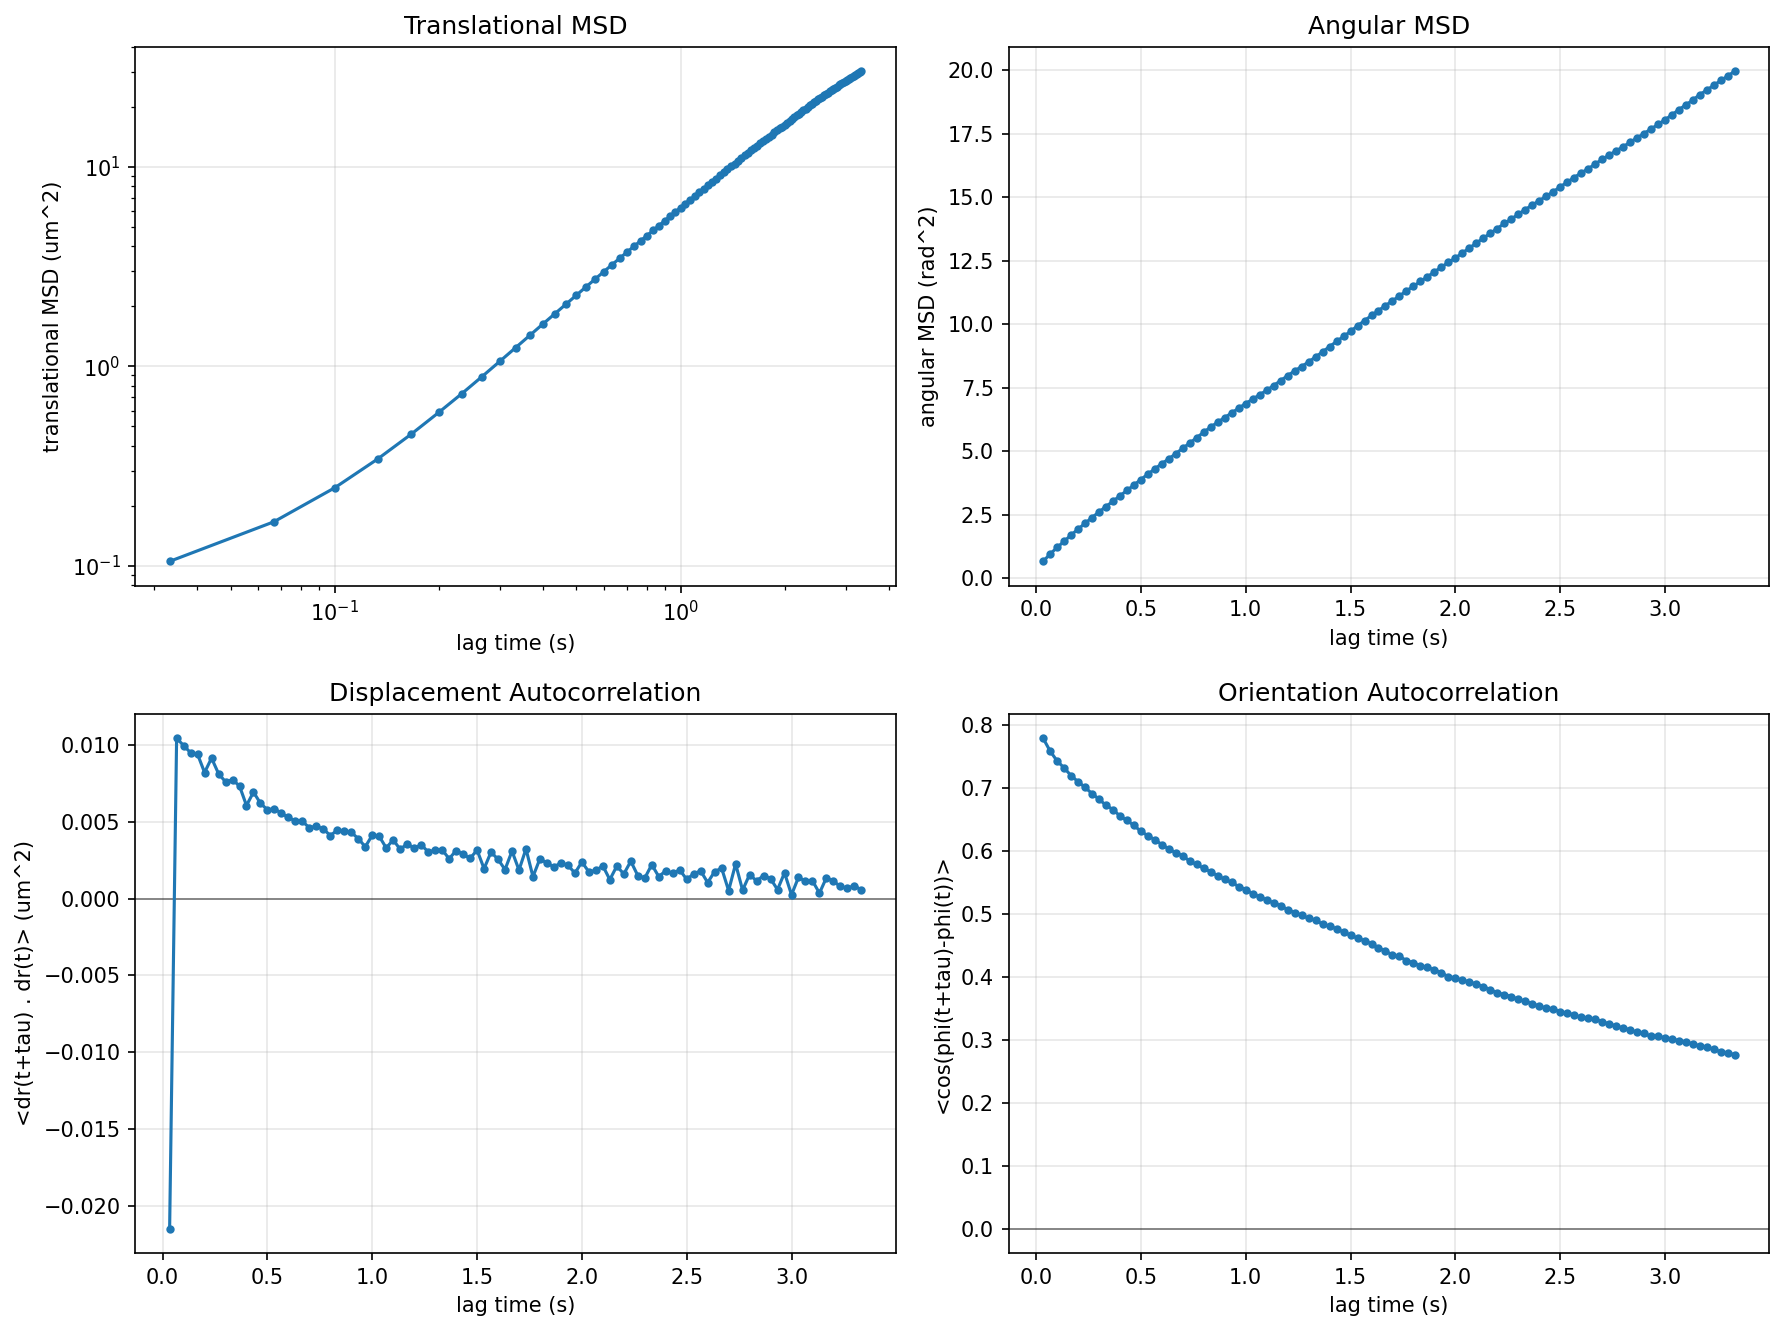
\includegraphics[width=\textwidth]{imglib/progress_update/motion_real_only_lag_statistics.png}
\end{figure}
\end{column}
\end{columns}
\end{frame}

\begin{frame}{Run \texttt{04}: Track-Derived Diagnostics}
\begin{columns}
\begin{column}{0.5\textwidth}
\begin{figure}
    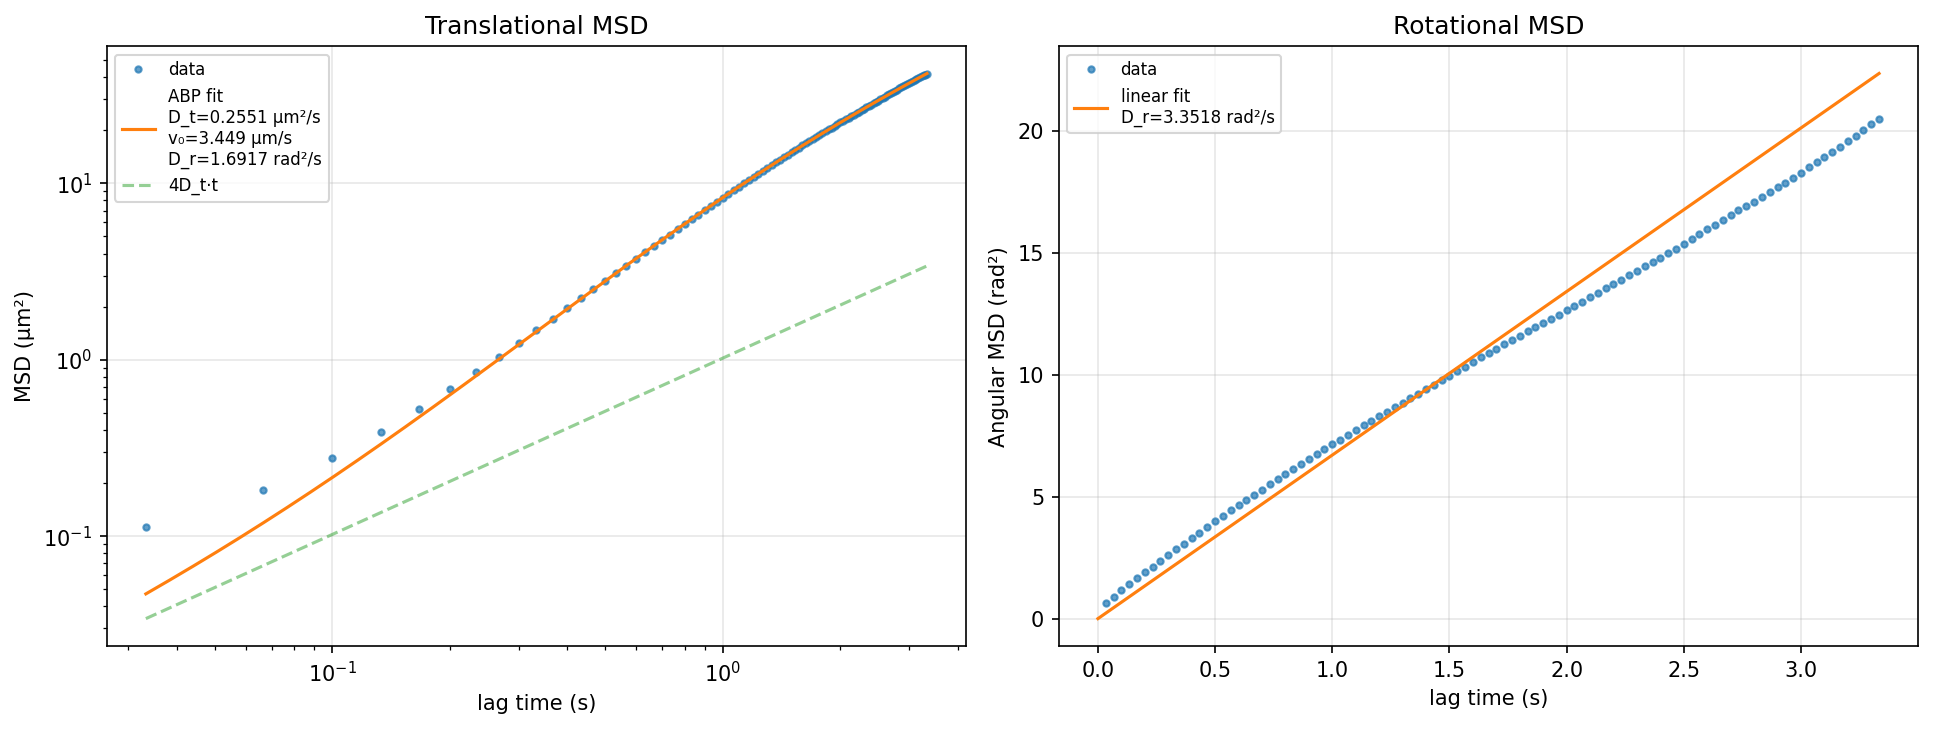
\includegraphics[width=\textwidth, height=0.70\textheight, keepaspectratio]{imglib/progress_update/run04_lodestar_tracks_msd.png}
\end{figure}
\end{column}
\begin{column}{0.5\textwidth}
\begin{figure}
    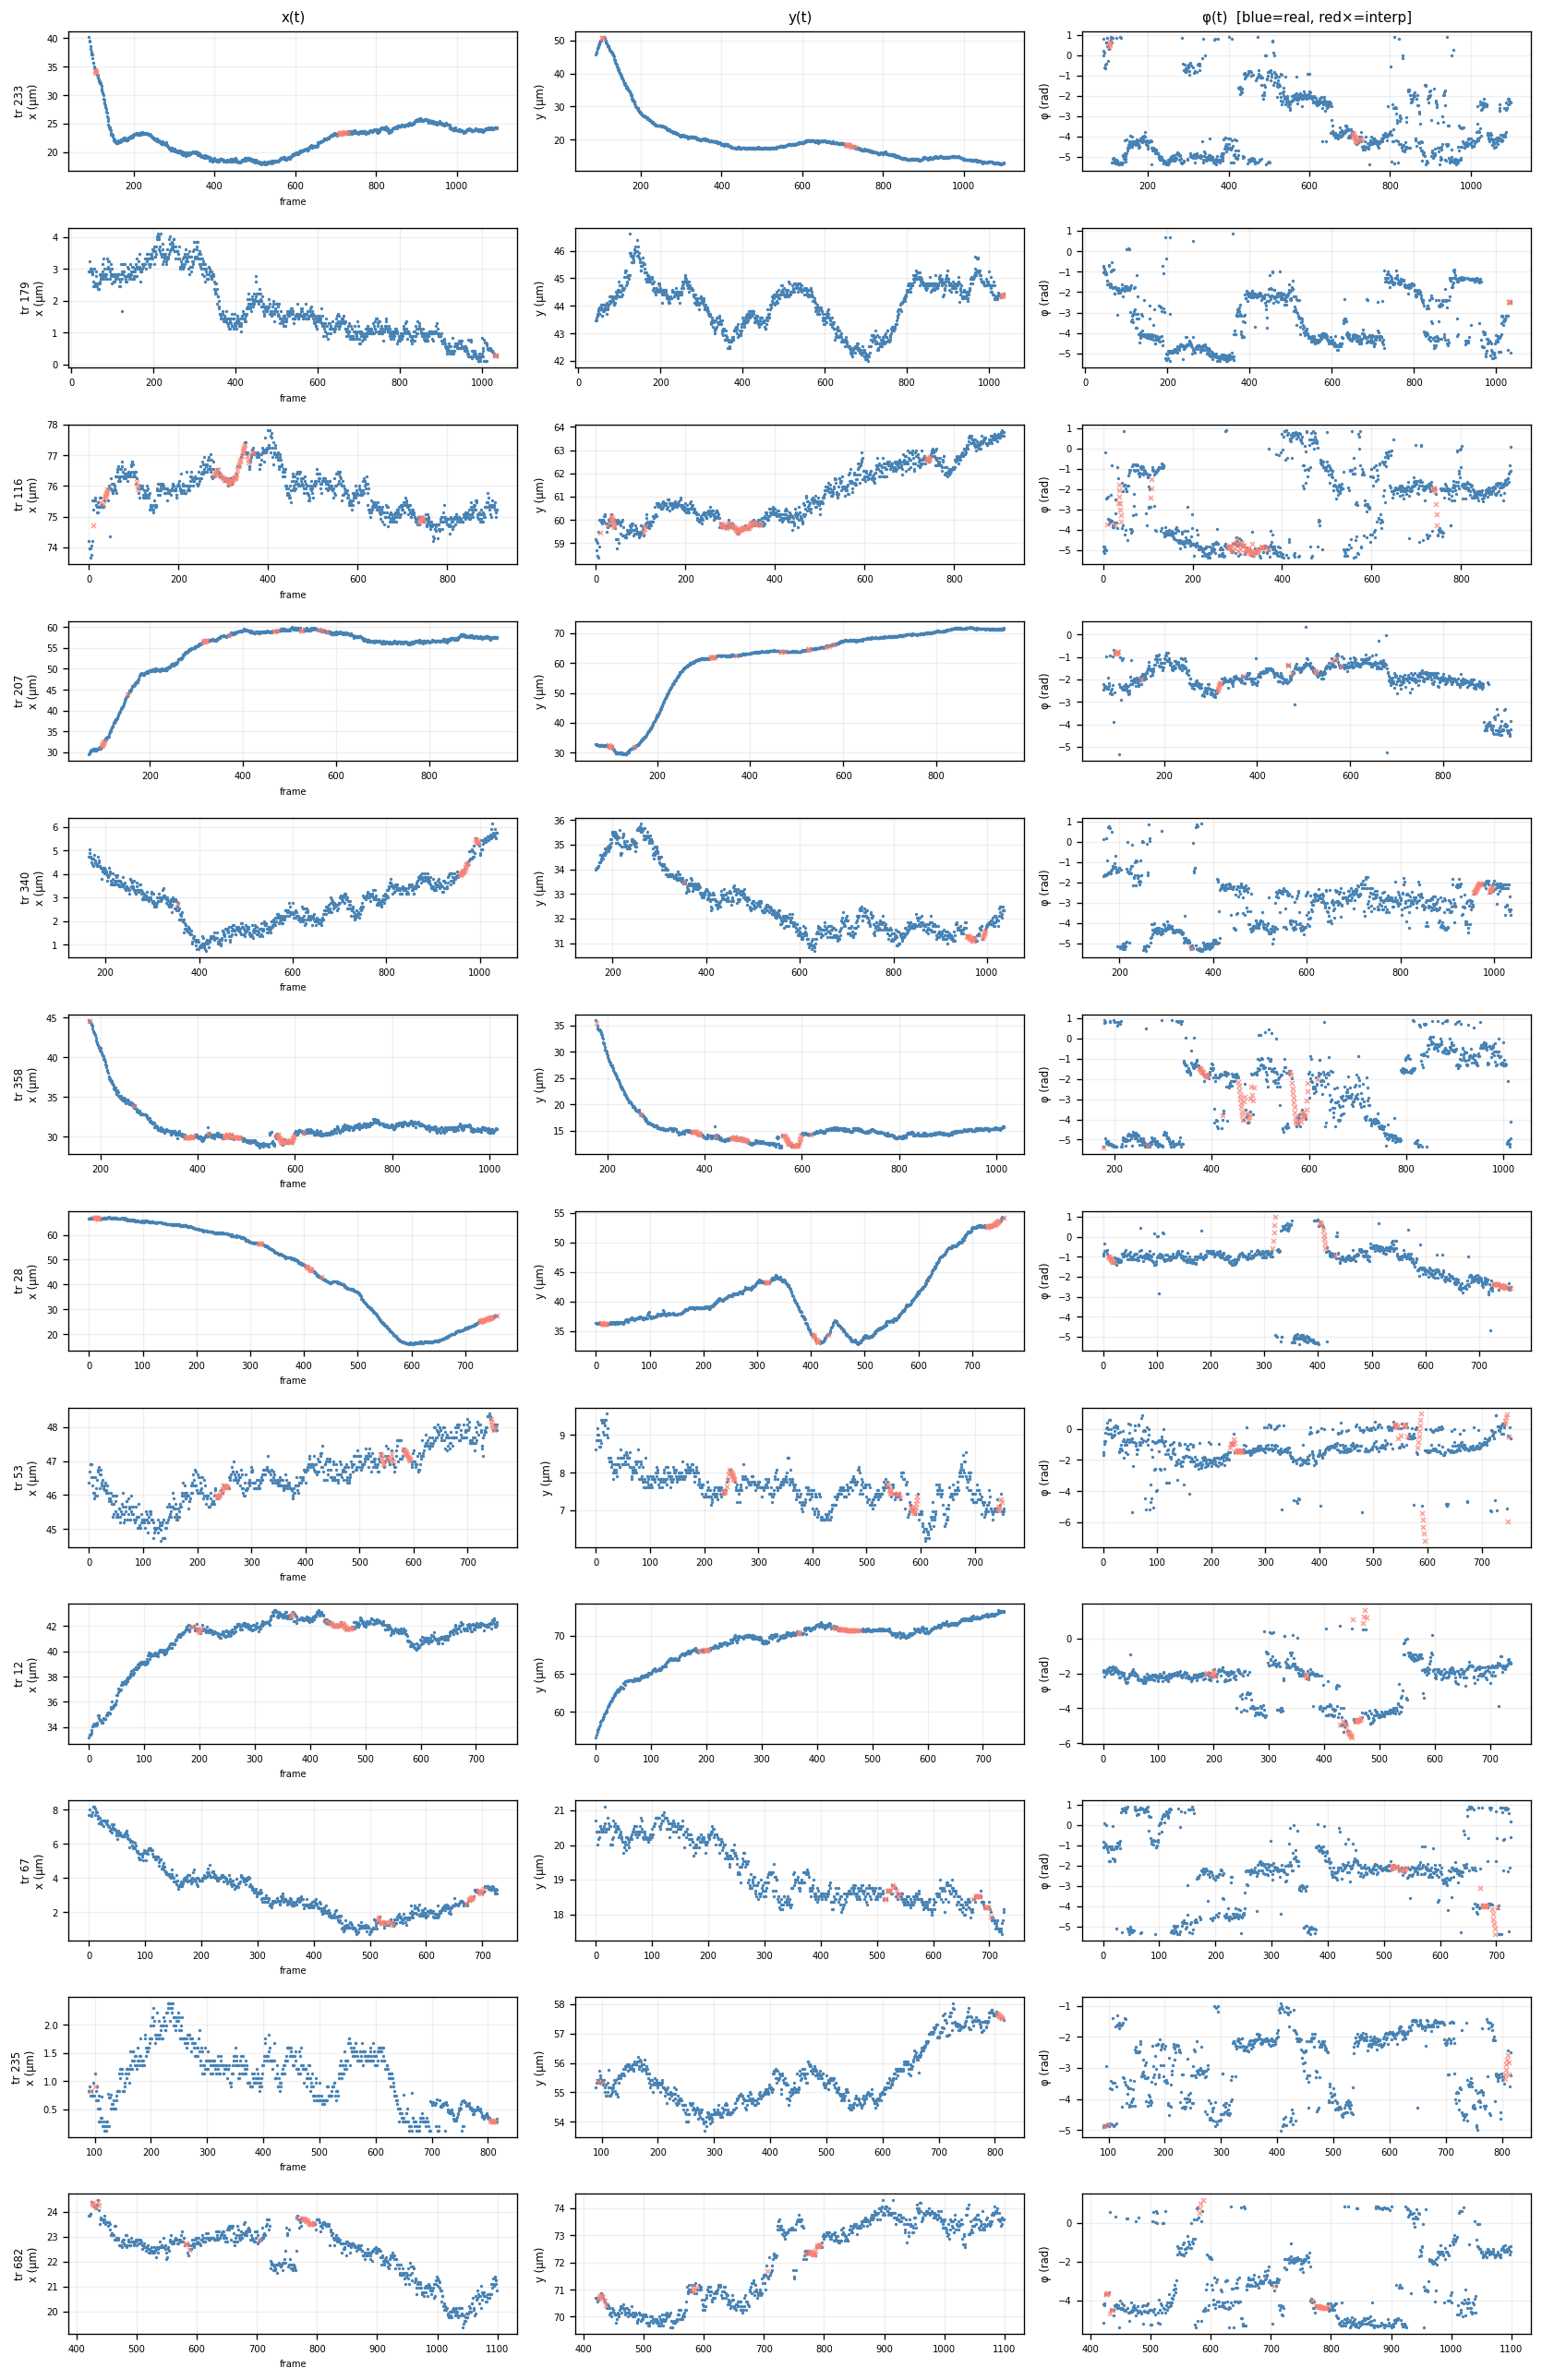
\includegraphics[width=\textwidth, height=0.70\textheight, keepaspectratio]{imglib/progress_update/run04_lodestar_sample_tracks.png}
\end{figure}
\end{column}
\end{columns}
\end{frame}

\begin{frame}{Run \texttt{04}: Analysis Outputs}
\begin{columns}
\begin{column}{0.5\textwidth}
\begin{figure}
    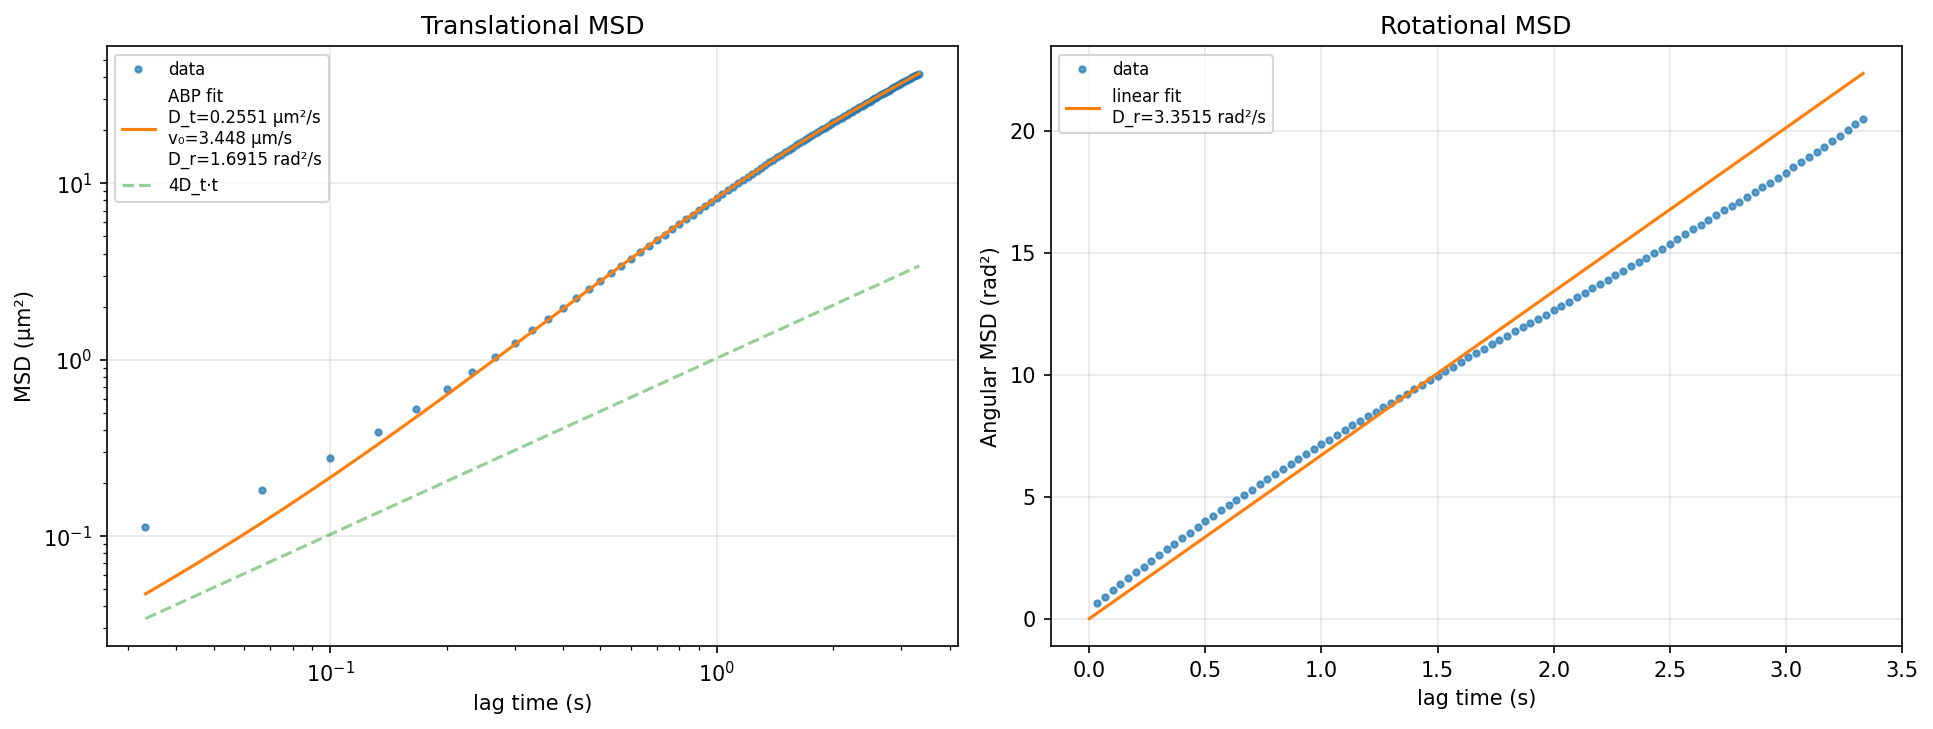
\includegraphics[width=\textwidth, height=0.70\textheight, keepaspectratio]{imglib/progress_update/run04_analysis_mona_slm075_msd.png}
\end{figure}
\end{column}
\begin{column}{0.5\textwidth}
\begin{figure}
    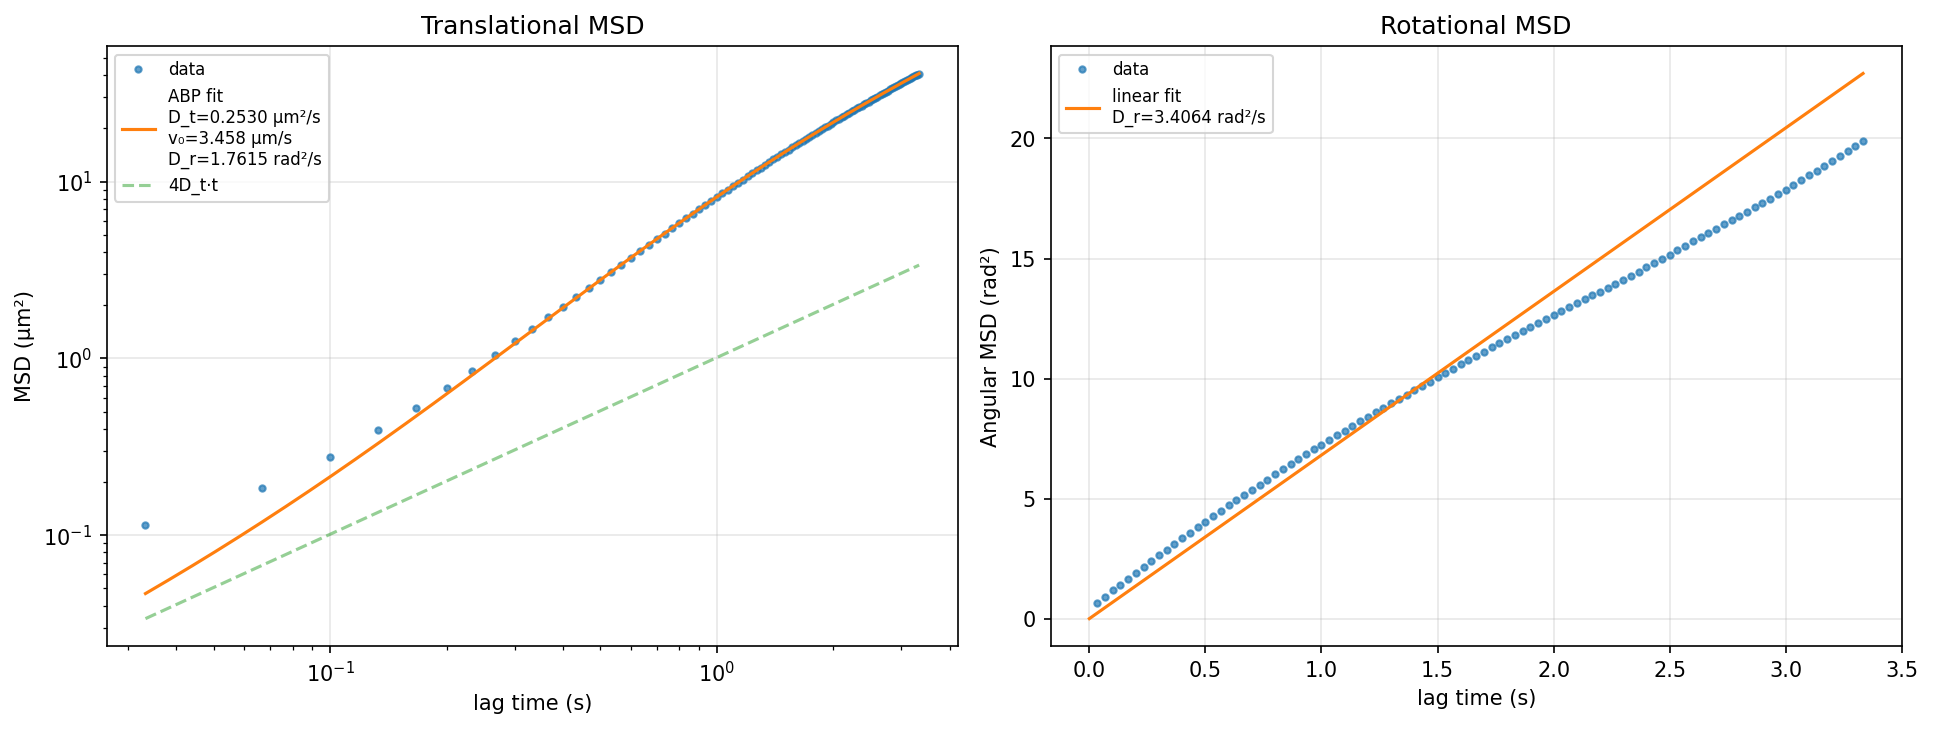
\includegraphics[width=\textwidth, height=0.70\textheight, keepaspectratio]{imglib/progress_update/run04_analysis_trackpy_slm075_msd.png}
\end{figure}
\end{column}
\end{columns}
\end{frame}
